\chapter{Introdução}

O interesse pela robótica educacional vem aumentando nas últimas décadas, uma vez que a mesma trás benefícios em todos os níveis da educação, seja no ensino de crianças, adolescentes ou adultos \cite{alimisis}. Robótica tem sido utilizada para ajudar no aprendizado da matemática, ciências ou engenharia através de atividades práticas que envolvem a programação de robôs \cite{Benitti2012}. A programação de robôs educacionais oferece apoio para o ensino e aprendizagem de programação, principalmente para aqueles que estão iniciando a construção do pensamento computacional, com o propósito de usar o raciocínio lógico para estruturar soluções coerentes para problemas complexos \cite{Bombasar2015}.

Ambientes de programação de robôs são geralmente atrativos e lúdicos com a intenção de despertar o fascínio e a curiosidade dos estudantes pela programação \cite{ESILVA}. Segundo a reportagem~\citeonline{jornal}, o uso de ambientes de robótica nas escolas públicas do estado de Pernambuco tem aumentado o interesse dos estudantes pelas disciplinas de matemática e física, além de aumentar a criatividade, a sociabilidade, a concentração e o senso de coletividade.

O ambiente de programação LEGO MindStorms\footnote[1]{https://www.lego.com/en-us/mindstorms} é um exemplo de aplicação com essa finalidade; apresenta uma interface onde o aluno pode desenvolver o programa que controla o robô antes de executar o programa no robô. Um problema no uso da robótica educacional é o alto custo para adquirir equipamentos, como por exemplo, o robô MindStorms da LEGO. Uma alternativa para o uso de robôs é utilizar ambientes de robótica educacional baseados em simulação como o RoboMind\footnote[2]{http://robomind.net/}. Estes ambientes permitem a simulação passo a passo do robô na tela do computador, a partir da execução dos comandos do programa, ocasionando em uma melhor compreensão para o aluno \cite{Lessa2015}. 

Um problema dos ambientes de simulação de robôs é que estes não oferecem um mecanismo de verificação automática das soluções propostas por estudantes, ou seja, os programas escritos pelos alunos não são verificados quanto a sua corretude para o problema proposto, de modo que estudante e professor possam obter \textit{feedback} automático sobre o funcionamento dos programas. O atual mecanismo de verificação em ambientes de simulação de robôs virtuais ocorre através da observação dos passos do robô, o que pode tornar a tarefa demorada e trabalhosa. Além de onerosa, a verificação pode ser complexa. Por isso, métodos de verificação automática são tão importantes para determinar a corretude de um programa em diferentes perspectivas de maneira automatizada e rápida \cite{Duarte}. 

%Portanto, este trabalho propõe uma abordagem para a tradução automática de uma linguagem de programação de robôs para um modelo formal com o objetivo de fornecer a alunos e professores uma forma de apoio durante a programação nesses ambientes por meio de \textit{feedback} automático. Além disso, este trabalho contribui para a área da Engenharia de Software através da junção da educação com a verificação de sistemas de software, por meio da abordagem proposta para resolver o problema descrito em seguida


%\section{Problema de Pesquisa}

Não existem ambientes gratuitos de programação de robôs que oferecem a estudantes e professores um mecanismo de análise automática dos programas. O único ambiente de verificação para robôs é o Robomind Academy\footnote[3]{https://www.robomindacademy.com/}. Este ambiente além de ser pago, só permite a verificação dos mapas já cadastrados no sistema, que estão associados a desafios de programação fixados; não é possível realizar a verificação automática dos programas levando em consideração diferentes mapas e soluções para um determinado problema. Exemplos de problemas são: identificar se o robô encontra a saída de um labirinto; se o robô encontra um objeto no mapa; ou simplesmente se o robô termina sua execução (não executa um laço infinito).

%O RoboMind, mostrado na Figura \ref{fig:robomind}, é um ambiente de programação de robôs virtuais para o ensino e aprendizagem de robótica; possui uma interface com um espaço para a escrita dos programas e um outro espaço onde o aluno pode acompanhar a execução do robô em um mapa. Nesse ambiente, os programas são escritos na linguagem ROBO, uma linguagem educacional desenvolvida para a programação de robôs que oferece os principais comandos de programação: estruturas condicionais, estruturas de repetição, procedimentos e declaração de variáveis. O programa ROBO, ilustrado no lado esquerdo da Figura 1, movimenta o robô enquanto o objeto (beacon) não é detectado à sua frente: se não há nenhum obstáculo à sua frente, o robô avança uma célula (forward), caso contrário o robô recua uma célula (backward) e muda sua orientação para a direita (right).


%O presente trabalho propõe a verificação automática de robôs programados na linguagem ROBO considerando diferentes mapas e desafios utilizando a técnica de verificação de modelos. Os programas considerados em ROBO possuem uma quantidade finita de estados, portanto a técnica possibilita realizar análises completas neste contexto.

%Um dos problemas para realizar verificação de modelos é que não existe modelo formal para linguagens de programação de robôs. 

Em um trabalho anterior~\cite{nogueira} propomos a sistematização do processo de tradução dos programas escritos em ROBO para um modelo formal. Naquele trabalho é utilizado a verificação de modelos para automatizar a verificação de programas de robôs virtuais no ambiente RoboMind. Esta abordagem de verificação se dá por meio de algumas etapas como mostrado na Figura~\ref{fig:fluxograma}. É usado como entrada o programa escrito na linguagem ROBO e o mapa no qual o programa será executado. Um processo de tradução automática produz como saída a especificação formal do programa escrita na linguagem da álgebra de processos CSP (\textit{Communicatting Sequential Processes})~\cite{Cleaveland2018}. Através de um processo automático também é obtida a representação formal do mapa. A especificação formal do mapa e do robô são entradas do verificador de modelos FDR~\cite{Gibson} que é utilizado para verificar as propriedades do robô. Como exemplo de propriedade, temos se o programa possui \textit{deadlock}, ou seja, se o programa termina sua execução. 

\begin{figure}[h]
\centering
\caption{Visão geral da abordagem de verificação automática}
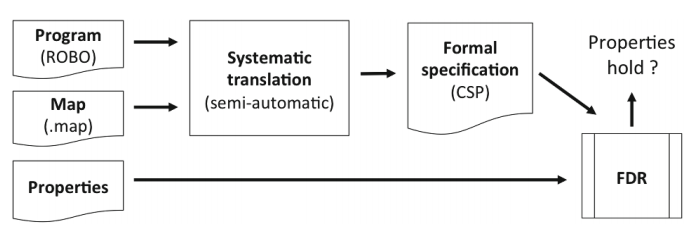
\includegraphics[height=5cm]{figuras/approach_workflow.png}
\fonte{\cite{nogueira}}
\label{fig:fluxograma}
\end{figure} 

%Em \cite{nogueira}, a especificação formal (ou modelo formal) é construída na linguagem de álgebra de processos CSP (\textit{Communicatting Sequential Processes}). CSP é uma ótima linguagem para expressar também a execução simultânea de vários robôs em um mesmo programa. Tal possibilidade não foi explorada por trabalhos disponíveis na literatura.

A maior complexidade da abordagem ilustrada na Figura \ref{fig:fluxograma} é a tradução da notação ROBO para a notação formal de CSP. Esta tradução é definida a partir de regras de mapeamento de cada elemento da linguagem ROBO para o seu equivalente em CSP; estas regras fazem parte de um compilador que automatiza a aplicação das regras. 
%No processo de criação do compilador, primeiro, as regras de mapeamento devem ser realizadas utilizando um \textit{framework} que contemple as etapas de criação de uma Linguagem de Domínio Específico (\textit{Domain-Specific Language} - DSL). As DSLs são linguagens de alto poder de abstração linguístico onde o desenvolvedor pode focar na lógica da aplicação, o que permite que elas possam ser automatizadas, analisadas e otimizadas. 
As etapas internas do compilador são: (1) criação de um \textit{parser} para a sintaxe da linguagem ROBO e (2) a geração do modelo CSP a partir da árvore sintática do programa usando regras de mapeamento. 
%; (5) integrar a linguagem dentro de um ambiente de desenvolvimento \cite{KatsSpoofax}. 
O \textit{framework} Spoofax~\cite{KatsSpoofax} foi utilizado para facilitar a implementação das etapas internas do compilador. 
%No contexto deste trabalho, a DSL corresponde a linguagem ROBO. Para esta DSL, a compilação deve considerar toda a sintaxe da linguagem ROBO, desde comandos padrões (condicionais e repetição) até mesmo declaração de variáveis e procedimentos. Para esta pesquisa o \textit{framework} Spoofax, o mesmo mostrado no artigo anterior, é adotado para realizar o mapeamento de ROBO para CSP, pois oferece um ambiente de desenvolvimento completo durante as etapas de compilação.

Atualmente, o compilador de ROBO para CSP não considera vários elementos importantes da linguagem como variáveis e procedimentos. Além disto, não existe uma integração do compilador com o verificador de modelos FDR. Também não existe uma interface que permita ao usuário utilizar a abordagem da Figura \ref{fig:fluxograma} de forma transparente. 

O presente trabalho estende a gramática do compilador para aceitar programas ROBO com variáveis e procedimentos, implementar regras de mapeamento de ROBO (que incluem variáveis e procedimentos) para CSP usando o \textit{framework} Spoofax  e integrar o compilador com FDR através de uma ferramenta que torne transparente para o usuário o processo de tradução e verificação.

%\section{Objetivos}
%Nesta seção estão dispostos os objetivos pretendidos por esta pesquisa.
%\subsection{Objetivo Geral}
%
%O trabalho proposto tem como objetivo a extensão e a automação de uma abordagem de tradução de uma linguagem através do desenvolvimento de um compilador com finalidade de realizar verificação automática de programas de robôs educacionais por meio de um modelo formal.
%
%\subsection{Objetivos Específicos}
%
%\begin{enumerate}
%    \item Definir regras de compilação para variáveis e procedimentos;
%    \item Estender o compilador existente da linguagem de programação ROBO para notação formal CSP;
%    \item Propor um protótipo funcional para análise de programas que integra o compilador com o verificador de modelos definido para este projeto.
%
%\end{enumerate}

%\section{Organização do Trabalho}

Os demais capítulos estão dispostos da seguinte maneira: o Capítulo \ref{chap:cap2} apresenta os aspectos teóricos utilizados ao longo desta pesquisa; o Capítulo \ref{chap:cap3} expõe a principal contribuição deste trabalho; no Capítulo \ref{chap:cap4} validamos a abordagem proposta por meio de um protótipo funcional; por fim, no Capítulo \ref{chap:cap5} são apresentados alguns trabalhos relacionados, além de expressar as considerações finais e expectativas para trabalhos futuros.